\section{Background}


\subsection{DVMS}

\subsubsection{Overview}
DVMS~\cite{quesnel:cpe12}
(\emph{Distributed Virtual Machine Scheduler}) is a framework that enables VMs
to be scheduled cooperatively and dynamically in large scale distributed
systems.

DVMS is deployed as a set of agents that are organized following a ring
topology and that cooperate with one another to guarantee the quality of
service~(QoS) for the VMs.

When a node cannot guarantee the QoS for its hosted VMs or when it is
under-utilized, it starts an iterative scheduling procedure~(ISP) by querying
its neighbor to find a better placement; it thus becomes the initiator of the ISP.
If the request cannot be satisfied by the neighbor, it is forwarded to the
following free one until the ISP succeeds.
This approach allows each ISP to send requests only to a minimal
number of nodes, thus decreasing the scheduling time without requiring a
central point.
In addition, this approach allows several ISPs to occur independently at the
same moment throughout the infrastructure; in other words, scheduling is
performed on partitions of the system that are created dynamically, which
significantly improves the reactivity of the system.
Communications are handled efficiently, as each node involved in a partition
can forward a request directly to the first node outside its partition, by
means of a ``first out'' relation.
\AL{FQ}{Ici il faut dire egalement que l'approche DVMS à la difference d'une approche gossip garantie de trouver une solution si il y en a une (absorbtion de tout le noeuds dans un microcosme). C'est important car le fait de basculer sur vivaldi ne remet pas en cause cette propriete (bien sure en evident la tolerance aux pannes mais vu qu'on en parle pas dans ce papier ca va)}
An example involving three partitions is shown on Figure~\ref{fig:isp}; in
particular, we can see the growth of partition~1 between two steps.
\begin{figure}[h!]
  \centering
  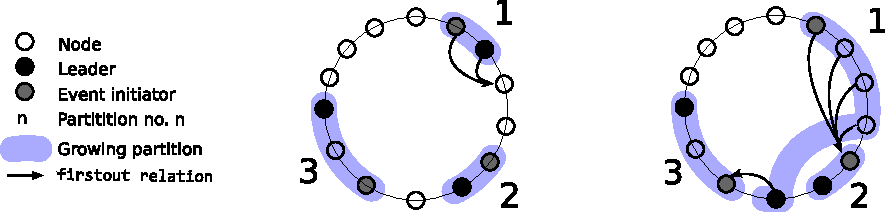
\includegraphics[width=0.9\linewidth]{Figures/resourceAcquisition-standard.pdf}
  \caption{Solving three problems simultaneously and independently with DVMS}%
  \label{fig:isp}%
\end{figure}

\subsubsection{Limitations}






\subsection{P2P - locality}


La prise en compte de la localit? dans la construction de r?seaux logiques
(\emph{overlays}) a ?t? initialement propos? dans le r?seau logique structur?
Pastry~\cite{pastry} afin d'optimiser la latence du routage. La recherche de ces
n\oe uds proches est fond?e sur un ?change p?diodique de r?f?rences de n\oe uds.

Le m?me concept a ?t? propos? dans les r?seaux logiques non structur?s afin de
permettre ? chaque n\oe ud de d?couvrir des n\oe uds du syst?mes les plus
\emph{proches}. La notion de proximit? peut recouvrir toute m?trique transitive
entre deux n\oe uds, en particulier le temps de latence entre les n\oe
uds~\cite{refquivabienmarindoittrouver}.

Le protocole Vivaldi~\cite{dabek:2001:sigcomm04}, sur lequel notre r?seau logique est fond?,
a une approche particuli?re. En effet, il fournit ? chaque n\oe ud des
coordonn?es dans un espace multi-dimensionnel refl?tant sa position dans le
r?seau physique. Initialement, chaque n\oe ud prend une position al?atoire de
l'espace, et choisit un petit sous-ensemble de n\oe uds. Puis, il se rapproche
dans l'espace, des n\oe uds avec lesquels il a une faible latence et s'?loigne
dans le cas inverse. Vivaldi ne permet donc pas de conna?tre les n\oe uds qui
lui sont proches dans le r?seau, mais de les reconna?tre via leurs coordonn?es.

Les approches pr?c?dentes maintiennent constamment la connaissance des n\oe udes
proches afin de fournir le meilleur n\oe ud possible, au co?t de communications
p?riodiques (ind?pendamment de la quantit? de requ?tes effectives.) Notre
approche se distingue par une approche paresseuse consistant ? rechercher des
n\oe uds proches (en s'appuyant sur les coordonn?es Vivaldi) lors des requ?tes,
adaptant ainsi la qualit? de la r?ponse ? la fr?quence des requ?tes.

